% Options for packages loaded elsewhere
\PassOptionsToPackage{unicode}{hyperref}
\PassOptionsToPackage{hyphens}{url}
%
\documentclass[
  10pt,
  brazil,
  a4paper,
  twoside, notitlepage, openright]{book}
\usepackage{lmodern}
\usepackage{amssymb,amsmath}
\usepackage{ifxetex,ifluatex}
\ifnum 0\ifxetex 1\fi\ifluatex 1\fi=0 % if pdftex
  \usepackage[T1]{fontenc}
  \usepackage[utf8]{inputenc}
  \usepackage{textcomp} % provide euro and other symbols
\else % if luatex or xetex
  \usepackage{unicode-math}
  \defaultfontfeatures{Scale=MatchLowercase}
  \defaultfontfeatures[\rmfamily]{Ligatures=TeX,Scale=1}
\fi
% Use upquote if available, for straight quotes in verbatim environments
\IfFileExists{upquote.sty}{\usepackage{upquote}}{}
\IfFileExists{microtype.sty}{% use microtype if available
  \usepackage[]{microtype}
  \UseMicrotypeSet[protrusion]{basicmath} % disable protrusion for tt fonts
}{}
\makeatletter
\@ifundefined{KOMAClassName}{% if non-KOMA class
  \IfFileExists{parskip.sty}{%
    \usepackage{parskip}
  }{% else
    \setlength{\parindent}{0pt}
    \setlength{\parskip}{6pt plus 2pt minus 1pt}}
}{% if KOMA class
  \KOMAoptions{parskip=half}}
\makeatother
\usepackage{xcolor}
\IfFileExists{xurl.sty}{\usepackage{xurl}}{} % add URL line breaks if available
\IfFileExists{bookmark.sty}{\usepackage{bookmark}}{\usepackage{hyperref}}
\hypersetup{
  pdftitle={Uso de R para análise dos dados da World Values Survey},
  pdfauthor={Tiago Vier, UFRGS; Daniel Capistrano, UCD; Jéssica Duarte, UFRGS; Luana Isabelle Beal, UFRGS; Carla Mendonça, ISCTE; Cristiana Verônica Mueller, UNISC},
  pdflang={pt-br},
  hidelinks,
  pdfcreator={LaTeX via pandoc}}
\urlstyle{same} % disable monospaced font for URLs
\usepackage[left=3cm,right=2cm,top=3cm,bottom=2cm]{geometry}
\usepackage{color}
\usepackage{fancyvrb}
\newcommand{\VerbBar}{|}
\newcommand{\VERB}{\Verb[commandchars=\\\{\}]}
\DefineVerbatimEnvironment{Highlighting}{Verbatim}{commandchars=\\\{\}}
% Add ',fontsize=\small' for more characters per line
\usepackage{framed}
\definecolor{shadecolor}{RGB}{248,248,248}
\newenvironment{Shaded}{\begin{snugshade}}{\end{snugshade}}
\newcommand{\AlertTok}[1]{\textcolor[rgb]{0.94,0.16,0.16}{#1}}
\newcommand{\AnnotationTok}[1]{\textcolor[rgb]{0.56,0.35,0.01}{\textbf{\textit{#1}}}}
\newcommand{\AttributeTok}[1]{\textcolor[rgb]{0.77,0.63,0.00}{#1}}
\newcommand{\BaseNTok}[1]{\textcolor[rgb]{0.00,0.00,0.81}{#1}}
\newcommand{\BuiltInTok}[1]{#1}
\newcommand{\CharTok}[1]{\textcolor[rgb]{0.31,0.60,0.02}{#1}}
\newcommand{\CommentTok}[1]{\textcolor[rgb]{0.56,0.35,0.01}{\textit{#1}}}
\newcommand{\CommentVarTok}[1]{\textcolor[rgb]{0.56,0.35,0.01}{\textbf{\textit{#1}}}}
\newcommand{\ConstantTok}[1]{\textcolor[rgb]{0.00,0.00,0.00}{#1}}
\newcommand{\ControlFlowTok}[1]{\textcolor[rgb]{0.13,0.29,0.53}{\textbf{#1}}}
\newcommand{\DataTypeTok}[1]{\textcolor[rgb]{0.13,0.29,0.53}{#1}}
\newcommand{\DecValTok}[1]{\textcolor[rgb]{0.00,0.00,0.81}{#1}}
\newcommand{\DocumentationTok}[1]{\textcolor[rgb]{0.56,0.35,0.01}{\textbf{\textit{#1}}}}
\newcommand{\ErrorTok}[1]{\textcolor[rgb]{0.64,0.00,0.00}{\textbf{#1}}}
\newcommand{\ExtensionTok}[1]{#1}
\newcommand{\FloatTok}[1]{\textcolor[rgb]{0.00,0.00,0.81}{#1}}
\newcommand{\FunctionTok}[1]{\textcolor[rgb]{0.00,0.00,0.00}{#1}}
\newcommand{\ImportTok}[1]{#1}
\newcommand{\InformationTok}[1]{\textcolor[rgb]{0.56,0.35,0.01}{\textbf{\textit{#1}}}}
\newcommand{\KeywordTok}[1]{\textcolor[rgb]{0.13,0.29,0.53}{\textbf{#1}}}
\newcommand{\NormalTok}[1]{#1}
\newcommand{\OperatorTok}[1]{\textcolor[rgb]{0.81,0.36,0.00}{\textbf{#1}}}
\newcommand{\OtherTok}[1]{\textcolor[rgb]{0.56,0.35,0.01}{#1}}
\newcommand{\PreprocessorTok}[1]{\textcolor[rgb]{0.56,0.35,0.01}{\textit{#1}}}
\newcommand{\RegionMarkerTok}[1]{#1}
\newcommand{\SpecialCharTok}[1]{\textcolor[rgb]{0.00,0.00,0.00}{#1}}
\newcommand{\SpecialStringTok}[1]{\textcolor[rgb]{0.31,0.60,0.02}{#1}}
\newcommand{\StringTok}[1]{\textcolor[rgb]{0.31,0.60,0.02}{#1}}
\newcommand{\VariableTok}[1]{\textcolor[rgb]{0.00,0.00,0.00}{#1}}
\newcommand{\VerbatimStringTok}[1]{\textcolor[rgb]{0.31,0.60,0.02}{#1}}
\newcommand{\WarningTok}[1]{\textcolor[rgb]{0.56,0.35,0.01}{\textbf{\textit{#1}}}}
\usepackage{longtable,booktabs}
% Correct order of tables after \paragraph or \subparagraph
\usepackage{etoolbox}
\makeatletter
\patchcmd\longtable{\par}{\if@noskipsec\mbox{}\fi\par}{}{}
\makeatother
% Allow footnotes in longtable head/foot
\IfFileExists{footnotehyper.sty}{\usepackage{footnotehyper}}{\usepackage{footnote}}
\makesavenoteenv{longtable}
\usepackage{graphicx,grffile}
\makeatletter
\def\maxwidth{\ifdim\Gin@nat@width>\linewidth\linewidth\else\Gin@nat@width\fi}
\def\maxheight{\ifdim\Gin@nat@height>\textheight\textheight\else\Gin@nat@height\fi}
\makeatother
% Scale images if necessary, so that they will not overflow the page
% margins by default, and it is still possible to overwrite the defaults
% using explicit options in \includegraphics[width, height, ...]{}
\setkeys{Gin}{width=\maxwidth,height=\maxheight,keepaspectratio}
% Set default figure placement to htbp
\makeatletter
\def\fps@figure{htbp}
\makeatother
\setlength{\emergencystretch}{3em} % prevent overfull lines
\providecommand{\tightlist}{%
  \setlength{\itemsep}{0pt}\setlength{\parskip}{0pt}}
\setcounter{secnumdepth}{5}
\usepackage{booktabs}
\usepackage[brazil]{babel}
\ifxetex
  % Load polyglossia as late as possible: uses bidi with RTL langages (e.g. Hebrew, Arabic)
  \usepackage{polyglossia}
  \setmainlanguage[]{brazil}
\else
  \usepackage[shorthands=off,main=brazil]{babel}
\fi
\usepackage[]{natbib}
\bibliographystyle{plainnat}

\title{Uso de R para análise dos dados da World Values Survey}
\author{Tiago Vier, UFRGS \and Daniel Capistrano, UCD \and Jéssica Duarte, UFRGS \and Luana Isabelle Beal, UFRGS \and Carla Mendonça, ISCTE \and Cristiana Verônica Mueller, UNISC}
\date{Coletivo WVSR, última atualização em 28/07/2020}

\begin{document}
\maketitle

{
\setcounter{tocdepth}{1}
\tableofcontents
}
\hypertarget{bem-vindoa}{%
\chapter*{Bem-Vindo(a)!}\label{bem-vindoa}}
\addcontentsline{toc}{chapter}{Bem-Vindo(a)!}

Este tutorial é resultado de um trabalho conjunto do Coletivo de Análises da World Values Survey (WVS), ou Pesquisa Mundial de Valores, em Português, sobre o uso da linguagem R e ambiente de programação RStudio.

Trata-se de um documento evolutivo e introdutório ao uso dos softwares livres R e RStudio nas análises dos dados da base estruturada da WVS.

Este tutorial foi preparado em \href{https://rmarkdown.rstudio.com/}{Rmarkdown} \citeyearpar{R-rmarkdown} com a biblioteca \href{https://bookdown.org/}{bookdown} \citeyearpar{R-bookdown}.

Um agradecimento aos colaboradores do grupo do WVS Brasil.

\hypertarget{intro}{%
\chapter{Introdução}\label{intro}}

\hypertarget{r-e-rstudio}{%
\section{R e RStudio}\label{r-e-rstudio}}

R é uma linguagem de programação com diversas características: tem como foco uma programação funcional, flexível, dinâmica e, principalmente, direcionada à manipulação, análise e visualização de dados.

É muito útil, por exemplo, para estudos de bases de dados complexas e pesquisas estatísticas. Essa funcionalidade também pode ser chamada de mineração de dados: o processo de exploração de dados em grande escala com o objetivo de buscar padrões, associações, relacionamentos e sistematização de variáveis.

O R e o RStudio são softwares livres e são compatíveis com os sistemas operacionais Windows, Linux e macOS, além de possuir boa integração com outros programas, como planilhas (por exemplo, Microsoft Excel) e outros softwares de análise de dados (por exemplo, SPSS).

O que justifica seu uso nas Ciências Sociais? Existe um uso crescente de métodos quantitativos nas Ciências Sociais acompanhado de uma maior disponibilidade de dados quantitativos. No entanto, cientistas sociais enfrentam diversas dificuldades de acesso às ferramentas tradicionais de análise de dados que são caras e oferecem pouco suporte para o aprendizado de estudantes e jovens pesquisadores. Além de contribuir para democratizar o uso de métodos quantitativos em Ciências Sociais, o R também tem o potencial de impulsionar a colaboração entre cientistas sociais e a reprodutibilidade de estudos na área.

\hypertarget{world-values-survey-wvs}{%
\section{World Values Survey (WVS)}\label{world-values-survey-wvs}}

A World Values Survey (WVS) investiga mudanças culturais em diversas sociedades e possibilita a comparação das características dessas mudanças, contribuindo, entre outros campos, para o debate sobre a relação entre desenvolvimento socio-econômico e mudanças culturais, para o acompanhamento longitudinal das mudanças em curso e para a ampliação do conhecimento de diferentes áreas do planeta -- muitas delas eram antes de acesso limitado a determinadas regiões.


\includegraphics{img/wvs_asso.jpg}

O embasamento teórico do WVS está associada à teoria da modernização e do pós-materialismo elaborada por Ronald Inglehart, que sugere que fenômenos como o crescimento do setor de serviços, a melhoria na qualidade de vida e o aumento das oportunidades educacionais nas sociedades industriais avançadas ou pós-industriais têm levado a uma gradual transformação nos valores e atitudes sociais.

A pesquisa teve início em 1981 e consiste em inquéritos representativos em nível nacional realizados em quase cem países, abrangendo quase 90\% da população mundial. Utiliza um questionário comum de 180 variáveis e inclui atualmente entrevistas com quase 400 mil indivíduos.

A tese articula duas hipóteses para explicar essa mudança:

\begin{enumerate}
\def\labelenumi{\alph{enumi})}
\tightlist
\item
  a \emph{hipótese da escassez}: defende que as prioridades da ação humana são resultado do ambiente sócio-econômico vigente, no qual valoriza-se subjetivamente coisas e aspectos da realidade que são escassos; e\\
\item
  \emph{hipótese da socialização}: defende que grande parte dos valores básicos de um indivíduo derivam das condições presentes em seu período de formação, anterior à idade adulta.
\end{enumerate}

Dessa forma, o WVS se desenvolve a partir de um referencial teórico específico mas possibilita uma ampla gama de análises. A pesquisa utiliza como hipótese central que \emph{``as mudanças nos sistemas de crenças de massas têm consequências sociais, políticas e econômicas importantes\emph{. Mas, ao mesmo tempo, }{[}\ldots{]} esta pesquisa proporciona outras análises a partir de seus resultados, haja vista a qualidade e a diversidade das dimensões e perguntas presentes no questionário.''} \citep{castro_conteudo_2015}


\includegraphics{img/wvs_logo.png}

O Brasil participou de cinco das sete ondas da WVS realizadas até agora (1990-1994; 1995-1999; 2005-2009; 2010-2014; e 2017-2020). O professor Henrique Castro coordena a pesquisa no país desde a quinta onda que foi baseada na Universidade de Brasília, entre 2005 e 2014, e a partir da Universidade Federal do Rio Grande do Sul (UFRGS), desde 2017, com financiamento da Capes/MEC.

O WVS no Brasil utiliza uma amostra probabilística completa em três etapas: a) seleção aleatória e estabelecimento de 150 clusters (baseada nos setores censitários do país, incluindo zonas urbanas e rurais); b) seleção aleatória de habitações em cada setor censitário; e c) escolha do entrevistado na habitação, considerando que seja alfabetizado, tenha 16 anos ou mais de idade e data de aniversário mais próxima do dia da primeira visita bem-sucedida.

Atualmente, o grupo de pesquisa WVS Brasil é integrado por discentes e docentes do Programa de Pós-Graduação em Ciência Política e discentes do Departamento de Economia e Relações Internacionais, ambos da UFRGS, e por pesquisadores de diversas universidades do Brasil, como Universidade de Brasília, Unisinos e Universidade de Caxias do Sul, e do Exterior, como a University College Dublin, integrando uma equipe de cerca de 60 pesquisadores.

Os dados gerados por todos os países integrantes da WVS ficam disponíveis para livre acesso na internet, por meio da página \url{www.worldvaluessurvey.org}.

\hypertarget{instalando-o-r-e-o-rstudio}{%
\chapter{Instalando o R e o RStudio}\label{instalando-o-r-e-o-rstudio}}

Para trabalhar com R, é necessário instalar dois softwares: R-base e RStudio. Para utilizar o RStudio, é necessário primeiro instalar o R-base.

Siga os passos para instalação de acordo com o sistema operacional do seu computador.

\hypertarget{linux}{%
\section{LINUX}\label{linux}}

\hypertarget{instalar-o-r}{%
\subsection{Instalar o R}\label{instalar-o-r}}

\begin{itemize}
\tightlist
\item
  Passo 1: Abra o terminal. Se utilizar distribuição Fedora, pressione as teclas Super + T, e no Ubuntu Ctrl + Alt + t;\\
\item
  Passo 2: Com o terminal aberto digite a seguinte linha de comando:

  \begin{itemize}
  \tightlist
  \item
    Fedora: \texttt{sudo\ dnf\ install\ R}
  \item
    Ubuntu: \texttt{sudo\ apt-get\ install\ r-base\ r-base-core}\\
  \end{itemize}
\item
  Passo 3: Pressione a tecla Enter para confirmar;\\
\item
  Passo 4: Digite a senha do usuário;\\
\item
  Passo 5: Clique em Confirmar. Pronto! O R estará instalado e pode ser acessado.
\end{itemize}

Link para eventual consulta: \url{http://cran-r.c3sl.ufpr.br/bin/linux/}

\hypertarget{instalar-o-rstudio}{%
\subsection{Instalar o RStudio}\label{instalar-o-rstudio}}

\begin{itemize}
\tightlist
\item
  Passo 1: Acesse o site \url{https://rstudio.com/products/rstudio/download/}\\
\item
  Passo 2: Encontre na página o local de download gratuito conforme figura abaixo:
\end{itemize}

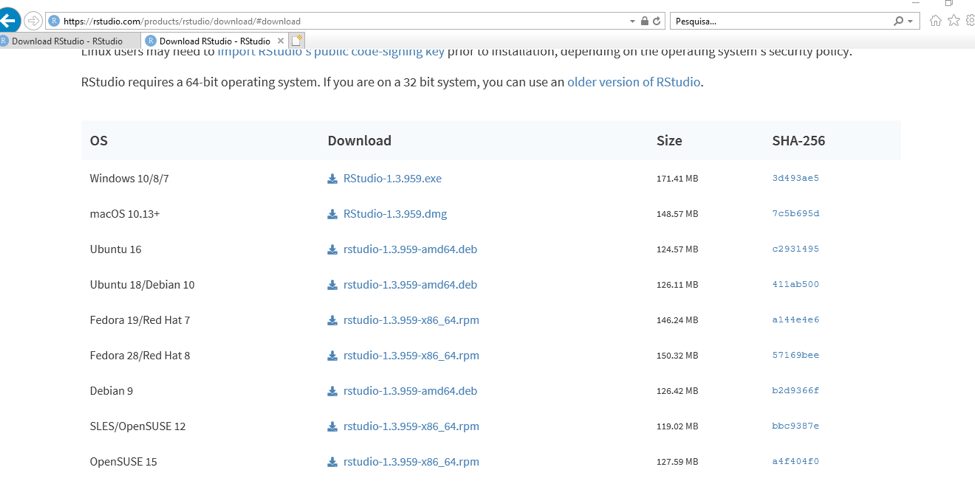
\includegraphics[width=13.54in]{img/inst_1_rstudio}

\begin{itemize}
\tightlist
\item
  Passo 3: Encontre o sistema operacional do seu computador (Ubuntu, Fedora, Debian ou OpenSUSE) e faça download.\\
\item
  Passo 4: Acesse o terminal na pasta onde foi feito o download e siga as instruções abaixo usando Fedora ou Ubuntu:

  \begin{itemize}
  \tightlist
  \item
    Fedora: \texttt{sudo\ dnf\ install\ nomedo\_arquivo\_baixado.rpm}; Ex: \texttt{sudo\ dnf\ install\ rstudio-1.3.959-x86\_64.rpm}
  \item
    Ubuntu: \texttt{sudo\ dpkg\ -i\ nomedo\_arquivo\_baixado.deb}\\
  \end{itemize}
\item
  Passo 5: O RStudio está instalado e pronto para uso!
\end{itemize}

\hypertarget{mac-os-x}{%
\section{Mac OS X}\label{mac-os-x}}

\hypertarget{instalar-o-r-1}{%
\subsection{Instalar o R}\label{instalar-o-r-1}}

\begin{itemize}
\tightlist
\item
  Passo 1: Abra o site \href{https://cran.r-project.org/}{CRAN - https://cran.r-project.org/}
\item
  Passo 2: Clique em ``Download de R for (Mac) OS X''.\\
\item
  Passo 3: Clique duas vezes no arquivo depois de baixado. Pronto! O R está instalado.
\end{itemize}

\hypertarget{instalar-o-rstudio-1}{%
\subsection{Instalar o RStudio}\label{instalar-o-rstudio-1}}

\begin{itemize}
\tightlist
\item
  Passo 1: Acesse o site \url{https://rstudio.com/products/rstudio/download/}\\
\item
  Passo 2: Encontre na página o local de download gratuito conforme figura abaixo:
\end{itemize}

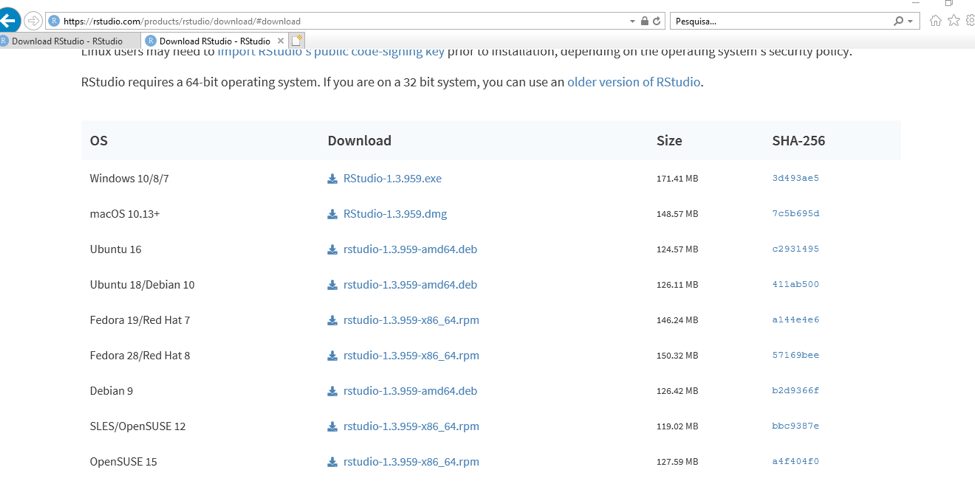
\includegraphics[width=13.54in]{img/inst_1_rstudio}

\begin{itemize}
\tightlist
\item
  Passo 3: Encontre o sistema operacional do seu computador (Mac OS) e faça download.\\
\item
  Passo 4: Depois de baixado, clique duas vezes no arquivo para instalá-lo. O RStudio está instalado e pronto para uso!
\end{itemize}

\hypertarget{windows}{%
\section{Windows}\label{windows}}

\hypertarget{instalar-o-r-2}{%
\subsection{Instalar o R}\label{instalar-o-r-2}}

\begin{itemize}
\tightlist
\item
  Passo 1: Clique no seguinte link \url{https://cran.r-project.org/bin/windows/base/}\\
\item
  Passo 2: Clique em Download R for Windows (os números que aparecem nesse arquivo de download correspondem à versão do R disponível):
\end{itemize}

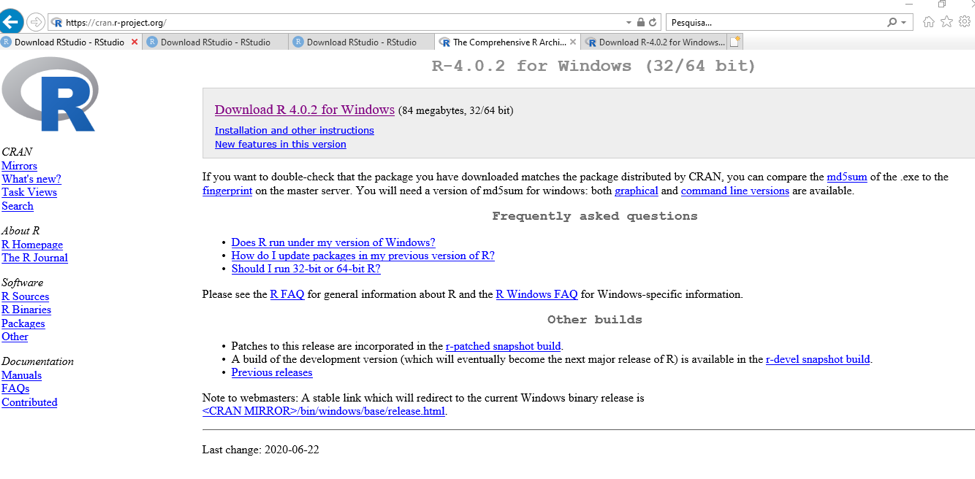
\includegraphics[width=13.54in]{img/inst_1_rwindows}

\begin{itemize}
\tightlist
\item
  Passo 3: Clique duas vezes no arquivo depois de baixado. Clique em Avançar até finalizar a instalação. Pronto! O R está instalado.
\end{itemize}

\hypertarget{instalar-o-rstudio-2}{%
\subsection{Instalar o RStudio}\label{instalar-o-rstudio-2}}

\begin{itemize}
\tightlist
\item
  Passo 1: Acesse o site \url{https://rstudio.com/products/rstudio/download/}\\
\item
  Passo 2: Encontre na página o local de download gratuito conforme figura abaixo:
\end{itemize}

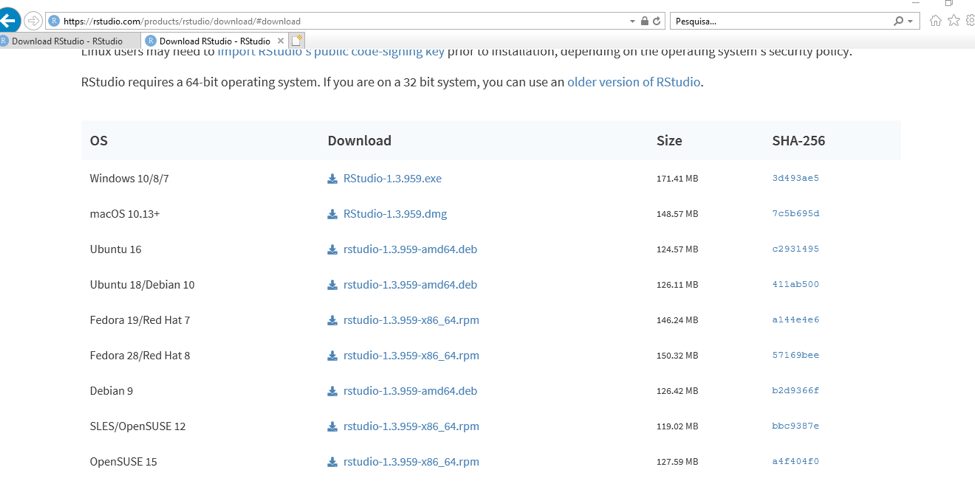
\includegraphics[width=13.54in]{img/inst_1_rstudio}

\begin{itemize}
\tightlist
\item
  Passo 3: Encontre o sistema operacional do seu computador (Windows) e faça download.
\item
  Passo 4: Depois de baixado, clique duas vezes no arquivo para instalá-lo. O RStudio está instalado e pronto para uso!
\end{itemize}

\hypertarget{identificando-o-rstudio}{%
\section{Identificando o RStudio}\label{identificando-o-rstudio}}

O RStudio tem quatro interfaces, espaços distribuídos na sua tela, fáceis de identificar e de trabalhar.

São elas:

\begin{itemize}
\tightlist
\item
  Source: local onde são inseridos os códigos-fonte. Fica no canto superior esquerdo.
\item
  Console: também chamado de terminal, onde são mostrados os resultados dos comandos executados pelos códigos na Source. Fica no canto inferior esquerdo.
\item
  Environment: também chamado de ambiente, onde são mostrados os elementos (por exemplo, vetores, bases de dados etc) que foram criados. Fica no canto superior direito.
\item
  Viewer: também chamado files, onde são mostrados os arquivos, pacotes, pastas, entre outros. Fica no canto inferior direito.
\end{itemize}

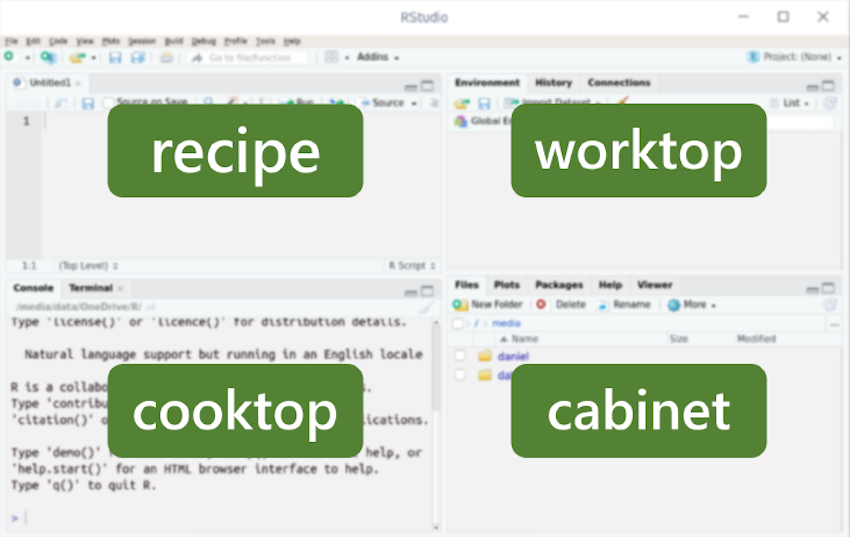
\includegraphics[width=11.81in]{img/cozinha}

\hypertarget{criando-um-projeto-no-rstudio}{%
\section{Criando um projeto no RStudio}\label{criando-um-projeto-no-rstudio}}

Uma forma prática de iniciar o trabalho com o RStudio é criando projetos.

Para iniciar um novo projeto:

\begin{itemize}
\tightlist
\item
  Acesse o menu ``File \textgreater{} New Project'', ou
\item
  então o ícone 
\includegraphics{img/proj_ico.png} na parte superior direita do RStudio.
\end{itemize}

O RStudio vai perguntar se você quer criar um novo diretório para o projeto, usar um diretório existente, ou ainda clonar um repositório distante (GitHub, por exemplo).

Para criar um novo diretório:

\begin{itemize}
\tightlist
\item
  Clique em ``New Directory'', escolha entre as opções de tipos de projeto oferecidas e dê um nome ao seu novo diretório.
\end{itemize}

Ali, você poderá salvar todos os documentos do projeto.

Ao fechar o RStudio, todos os documentos e os objetos do ambiente serão salvos no projeto, e você pode retomar o trabalho de onde parou quando quiser.

Lembre-se: as bibliotecas devem ser recarregadas cada vez que você iniciar uma seção do R.

\hypertarget{biblio}{%
\chapter{Bibliotecas}\label{biblio}}

Quando instalamos o R, instalamos junto uma grande quantidade de comandos e funções. A lista de funções do R-base pode ser vista \href{https://stat.ethz.ch/R-manual/R-devel/library/base/html/00Index.html}{aqui}.

Para além desses recursos, o R dispõe de uma grande quantidade de bibliotecas (ou pacotes). No momento em que escrevemos este tutorial, a plataforma de contribuições \href{https://cran.r-project.org/web/packages/}{CRAN} lista 16,045 bibliotecas disponíveis. As diferentes contribuições são agrupadas por tópicos. É possível, por exemplo, conhecer os pacotes disponíveis para as \href{https://cran.r-project.org/web/views/SocialSciences.html}{Ciências Sociais}.

Neste tutorial, utilizamos as funções do R-base e sugerimos bibliotecas adicionais que facilitam algumas operações e são suficientes para a maior parte das necessidades de um pesquisador interessado em analisar os dados do WVS.

As bibliotecas que são usadas neste tutorial fazem parte do grupo de pacotes \href{https://www.tidyverse.org/}{tidyverse} \citeyearpar{R-tidyverse}. Entre elas, estão os pacotes dplyr, haven e ggplot2. Mais detalhes sobre esse tema podem ser obtidos no livro acessível \href{https://r4ds.had.co.nz/}{neste link}. Além do \texttt{tidyverse}, usamos a biblioteca \texttt{codebook} para ter acesso ao metadados disponíveis nos arquivos de SPSS e Stata.

\hypertarget{instalando-bibliotecas-adicionais}{%
\section{Instalando bibliotecas adicionais}\label{instalando-bibliotecas-adicionais}}

Como mencionamos anteriormente, quando instalamos o R-base já instalamos uma série de funções e comandos.

Entretanto, você pode usar um comando específico para instalar novas bibliotecas do repositório CRAN.

Para instalar bibliotecas, use o comando: \texttt{install.packages("nome\_da\_bibliteca")}.

Outra maneira de instalar novas bibliotecas é usar a aba ``Packages''.

Essa aba permite visualizar as bibliotecas já instaladas e instalar novas usando o botão ``Install''.

Para instalar a biblioteca tidyverse digite:

\begin{Shaded}
\begin{Highlighting}[]
\CommentTok{# para instalar as bibliotecas da tidyverse}
\KeywordTok{install.packages}\NormalTok{(}\StringTok{"tidyverse"}\NormalTok{)}
\end{Highlighting}
\end{Shaded}

Para instalar a biblioteca codebook de visualização de metadados (ver no capítulo seguinte) digite:

\begin{Shaded}
\begin{Highlighting}[]
\CommentTok{# para instalar a biblioteca codebook para visualizar os metadados }
\CommentTok{# (ver no capítulo seguinte)}
\KeywordTok{install.packages}\NormalTok{(}\StringTok{"codebook"}\NormalTok{)}
\end{Highlighting}
\end{Shaded}

Quando rodamos o comando, usando \texttt{Crtl\ +\ Enter} ou \texttt{Run} no script, ou \texttt{Enter} se você está digitando diretamente no console, o R vai verificar se existem dependências e instalar todas as que forem necessárias para o seu funcionamento.

\textbf{É importante que se instale todas as dependências indicadas pelo R.} Verifique no Console e, se o R perguntar se você quer fazer a instalação das dependências, selecione ``Yes''.

\hypertarget{carregando-bibliotecas}{%
\section{Carregando bibliotecas}\label{carregando-bibliotecas}}

É preciso carregar as bibliotecas sempre que se inicia uma nova sessão.

O comando para carregar as bibliotecas é \texttt{library("nome\_da\_biblioteca")}.

Para carregar as bibliotecas que vamos usar, use os comandos abaixo:

\begin{Shaded}
\begin{Highlighting}[]
\CommentTok{# carregar o tidyverse}
\KeywordTok{library}\NormalTok{(tidyverse)}

\CommentTok{# carregar a biblioteca haven, }
\CommentTok{# usada para importar o arquivo  no formato do SPSS }
\KeywordTok{library}\NormalTok{(haven)}

\CommentTok{# carregar o codebook}
\KeywordTok{library}\NormalTok{(codebook)}
\end{Highlighting}
\end{Shaded}

Sempre que abrir o RStudio, é preciso recarregar as bibliotecas, pois o RStudio reinicia a sessão somente com os comandos do R-base.

É recomendado que as bibliotecas que serão usadas nas análises sejam indicadas no início do código R onde são feitas as análises. Dessa forma, qualquer pesquisador poderá identificar os requisitos necessários para reproduzir as suas análises.

Uma vez carregadas as bibliotecas, nós podemos continuar para o próximo passo que é importar os dados que vamos analisar.

\hypertarget{importando-bases-de-dados}{%
\chapter{Importando bases de dados}\label{importando-bases-de-dados}}

Utilizando o RStudio, pode-se abrir arquivos salvos no formato do próprio R (.RData) e de variados outros softwares, como Excel(.xlsx), SPSS (.sav) e Stata (.dta), e em diversos outros formatos, incluindo texto e csv.

Há duas formas de abrir arquivos de dados no RStudio:

\begin{itemize}
\tightlist
\item
  Com o uso do painel ``Environment'', ou
\item
  Com o uso de linhas de comando escritas diretamente no Console ou em um script
\end{itemize}

\hypertarget{com-o-uso-das-ferramentas-da-aba-environment}{%
\section{Com o uso das ferramentas da aba ``Environment''}\label{com-o-uso-das-ferramentas-da-aba-environment}}

Por essa forma, você usa as ferramentas do R do mesmo jeito que faz com qualquer outro software, como os do pacote Microsoft Office, por exemplo.

\hypertarget{arquivos-em-formato-r}{%
\subsection{Arquivos em formato R}\label{arquivos-em-formato-r}}

Para arquivos formato R (formato \texttt{.RData}):

\begin{itemize}
\tightlist
\item
  Na aba ``Environment'', clique sobre o icone ``Abrir Arquivos''.\\
\item
  Procure o seu arquivo nos locais do seu computador.\\
\item
  Clique no arquivo e clique em Open ou clique duas vezes sobre o arquivo.
\end{itemize}

Pronto! O seu arquivo vai aparecer no Environment.

\hypertarget{arquivos-em-outros-formatos}{%
\subsection{Arquivos em outros formatos}\label{arquivos-em-outros-formatos}}

Para importar os dados em outros formatos, é preciso ter bibliotecas específicas para esse fim. Neste tutorial, sugerimos que você tenha instalada e carregada a biblioteca haven, da gramática Tidyverse (veja em \protect\hyperlink{biblio}{bibliotecas}).

\begin{itemize}
\tightlist
\item
  Clique sobre o icone Import Dataset.
\item
  Escolha e clique sobre o formato em que o seu arquivo foi previamente salvo.
\item
  Clique em Browse.
\item
  Procure o seu arquivo nos locais do seu computador.
\item
  Clique no arquivo e clique em Open ou clique duas vezes sobre o arquivo.
\end{itemize}

Pronto! O seu arquivo vai aparecer no Environment.

\hypertarget{com-o-uso-de-linhas-de-comando}{%
\section{Com o uso de linhas de comando}\label{com-o-uso-de-linhas-de-comando}}

\hypertarget{arquivos-em-formato-r-1}{%
\subsection{Arquivos em formato R}\label{arquivos-em-formato-r-1}}

Para carregar arquivos no formato nativo do R usando linhas de comando:

\begin{itemize}
\tightlist
\item
  Abra um novo script R e digite: \texttt{load("nome\_do\_arquivo.rdata")}.

  \begin{itemize}
  \tightlist
  \item
    Dica: Deixe o cursor entre as aspas e tecle TAB. O R vai lhe mostrar os diretórios do seu computador. Se seu arquivo está em alguma pasta ou subpasta o R também vai lhe mostrar esses locais.\\
  \end{itemize}
\item
  Clique no arquivo que você quer importar\\
\item
  Digite Control + Enter, ou clique em Run (disponível na aba superior do Source Code do seu R).
\end{itemize}

Pronto! O seu arquivo vai aparecer no Environment.

\hypertarget{arquivos-em-outros-formatos-1}{%
\subsection{Arquivos em outros formatos}\label{arquivos-em-outros-formatos-1}}

Para importar os dados em outros formatos, é preciso ter bibliotecas específicas para esse fim. Neste tutorial, sugerimos que você tenha instalada e carregada a biblioteca \texttt{haven} da gramática Tidyverse (veja em \protect\hyperlink{biblio}{bibliotecas}).

Cada tipo de arquivo tem um comando específico na biblioteca \texttt{haven}:

Arquivos SPSS: função \texttt{read\_sav()}\\
Arquivos Excel: função \texttt{read\_csv()}\\
Arquivos Stata: função \texttt{read\_dta()}\\
Arquivos SAS: função \texttt{read\_sas()}

Para que a base se transforme em um objeto no Environment do R, é preciso que se atribua um nome a ele. Veja este exemplo com a extensão do SPSS (arquivos em formato .sav):

\begin{Shaded}
\begin{Highlighting}[]
\CommentTok{# carregar a biblioteca haven}
\KeywordTok{library}\NormalTok{(haven)}

\CommentTok{# abrir usando a função e criar um objeto no ambiente R}
\NormalTok{base_do_wvs <-}\StringTok{ }\KeywordTok{read_sav}\NormalTok{(}\StringTok{"diretório_do_projeto/nome_do_arquivo.sav"}\NormalTok{)}
\end{Highlighting}
\end{Shaded}

Como dito na dica anteriormente, deixe o cursor entre as aspas e tecle TAB. O R vai lhe mostrar os diretórios do seu computador. Em seguida, é só clicar sobre o arquivo que você procura.

\begin{itemize}
\tightlist
\item
  Tecle Control + Enter, ou\\
\item
  Clique em Run (disponível na aba superior do Source Code do seu R).
\end{itemize}

Pronto! O seu arquivo vai aparecer no Environment.

Com outras extensões você usará, por exemplo, \texttt{read\_cvs()} ou \texttt{read\_dta()}. Para mais informações acesse a \href{https://haven.tidyverse.org/}{ajuda da bibliteca haven}

\hypertarget{gerando-um-dicionuxe1rio-de-variuxe1veis}{%
\section{Gerando um dicionário de variáveis}\label{gerando-um-dicionuxe1rio-de-variuxe1veis}}

Para navegar na base de dados recém importada e reconhecer as variáveis importadas e suas características, existem diversas ferramentas disponíveis.

Uma delas é o pacote \texttt{codebook}, que gera um dicionário de variáveis. Nos exemplos abaixo, mostramos como gerar um dicionário de variáveis estático na aba ``Preview'' e também na forma de um objeto que pode ser visualizado como uma tabela.

Para carregar a biblioteca codebook e gerar um dicionário de variáveis estático navegável na aba ``Preview'', gerar uma tabela e visualisá-la use os comandos abaixo:

\begin{Shaded}
\begin{Highlighting}[]
\CommentTok{# carregar a biblioteca codebook}
\KeywordTok{library}\NormalTok{(codebook)}

\CommentTok{# gerar um dicionário de variáveis estático navegável na aba "Preview"}
\KeywordTok{label_browser_static}\NormalTok{(base_do_wvs)}

\CommentTok{# gerar uma tabela com todas as variávis}
\NormalTok{dicionario <-}\StringTok{ }\KeywordTok{codebook_table}\NormalTok{(base_do_wvs)}

\CommentTok{# visualizar na forma de tabela junto aos scripts R}
\KeywordTok{view}\NormalTok{(dicionario)}
\end{Highlighting}
\end{Shaded}

Feita a importação da base de dados e com o dicionário em mãos, podemos passar a descrição, análise e visualização dos dados.

\hypertarget{descrevendo-e-analisando-os-dados}{%
\chapter{Descrevendo e analisando os dados}\label{descrevendo-e-analisando-os-dados}}

Após instalar R e RStudio, reconhecer seu ambiente de trabalho, instalar e carregar as bibliotecas e importar os bancos de dados, começa a verdadeira diversão: finalmente, você vai trabalhar com os dados!

O R permite que se faça desde as operações mais simples, como uma calculadora, passando pela organização e limpeza dos dados, até análises estatísticas mais avançadas.

Um excelente começo dessa empreitada é a descrição dos dados que não só garante o divertimento do pesquisador, como também permite que se façam excelentes análises e conclusões.

A partir da estatística descritiva, obtém-se um conjunto de ferramentas que permitem:

\begin{enumerate}
\def\labelenumi{\alph{enumi})}
\tightlist
\item
  organizar os dados - agrupando, selecionando, filtrando, ordenando, criando variáveis;\\
\item
  descrever e analisar os dados - resumindo-os com base em sua média, moda, mediana, cruzando e contando as variáveis, criando gráficos e tabelas.
\end{enumerate}

A principal função da estatística descritiva é resumir os dados e facilitar a assimilação da informação \citep{agresti_metodos_2012}.

Além da descrição dos dados, o R também oferece suporte para que sejam feitos testes estatísticos mais avançados bi e multivariados, entre eles, correlação e regressão linear múltipla que iremos discutir mais adiante.

Nesta seção, você pode aprender os comandos do R que permitem criar anotações, criar variáveis e vetores, conectar sentenças do código de programação, visualizar os valores máximo e mínimo de uma variável, obter a média, somar os valores de uma variável, filtrar, selecionar, ordenar, contar, cruzar, criar nova coluna, resumir os dados a partir de alguma operação, excluir valores da análise, visualizar variáveis, fazer gráficos, fazer testes de correlação e análises de regressão multivariada.

Isso é tudo o que se precisa para, em ordem de importância: ter adoráveis momentos com o seu banco de dados e construir conhecimento a partir de análises robustas.

\hypertarget{descrevendo-os-dados}{%
\section{Descrevendo os dados}\label{descrevendo-os-dados}}

\hypertarget{criar-variuxe1veis-e-vetores}{%
\subsection{Criar variáveis e vetores}\label{criar-variuxe1veis-e-vetores}}

Para criar uma variável, escolha um nome para ela e atribua através do sinal \texttt{\textless{}-} um valor para a mesma, lembrando sempre de que o R não aceita caracteres do tipo espaço, então se o nome de sua variável tiver mais de um termo é necessário usar o conector underline (\_) entre as palavras. Lembre-se também que o R faz a diferença entre letras maiúsculas e minúsculas.

Para criar vetores, segue-se a mesma lógica, mas os valores devem ser inseridos entre os parênteses do código: \texttt{c()}, o qual indica que há um conjunto de valores (esses valores devem ser separados por vírgulas e entre aspas no caso de o valor ser um caractere, ou \emph{string}). Os valores atribuídos podem ser números simples, podem ser operações como soma, subtração, multiplicação.

Após criados, variáveis e vetores, podem também ter seus valores submetidos a algum tipo de operação. Veja estes exemplos:

\begin{Shaded}
\begin{Highlighting}[]
\CommentTok{# Criar um vetor chamado "Meu_resultado" que é o resultado da operação 1 + 5}
\NormalTok{Meu_resultado <-}\StringTok{ }\DecValTok{1} \OperatorTok{+}\StringTok{ }\DecValTok{5}

\CommentTok{# Criar um vetor chamado "Brasil" e multiplicá-lo por 3}
\NormalTok{Brasil <-}\StringTok{ }\KeywordTok{c}\NormalTok{(}\DecValTok{1}\NormalTok{, }\DecValTok{3}\NormalTok{, }\DecValTok{10}\NormalTok{, }\DecValTok{12}\NormalTok{, }\DecValTok{19}\NormalTok{, }\DecValTok{21}\NormalTok{, }\DecValTok{28}\NormalTok{, }\DecValTok{30}\NormalTok{, }\DecValTok{37}\NormalTok{)}
\NormalTok{Brasil }\OperatorTok{*}\StringTok{ }\DecValTok{3}

\CommentTok{# Criar um vetor chamado Países com strings/textos}
\NormalTok{Paises <-}\StringTok{ }\KeywordTok{c}\NormalTok{(}\StringTok{"Argentina"}\NormalTok{, }\StringTok{"Brasil"}\NormalTok{) }

\CommentTok{# Cálculo da idade com base no ano de nascimento}
\NormalTok{Ano_Nasc <-}\StringTok{ }\KeywordTok{c}\NormalTok{(}\DecValTok{1990}\NormalTok{, }\DecValTok{1984}\NormalTok{, }\DecValTok{1961}\NormalTok{)}

\CommentTok{# Calcular as idades}
\DecValTok{2020} \OperatorTok{-}\StringTok{ }\NormalTok{Ano_Nasc}

\CommentTok{# Armazenar como um vetor na aba Environment}
\NormalTok{Idade <-}\StringTok{ }\DecValTok{2020} \OperatorTok{-}\StringTok{ }\NormalTok{Ano_Nasc}
\end{Highlighting}
\end{Shaded}

\hypertarget{funuxe7uxf5es-buxe1sicas-e-comandos-uxfateis}{%
\subsection{Funções básicas e comandos úteis}\label{funuxe7uxf5es-buxe1sicas-e-comandos-uxfateis}}

Após carregar seu banco de dados ou criar suas próprias variáveis, é possível começar a conhecer e operar os dados observando seus valores máximos, mínimos, média e efetuando operações a partir dos valores dentro da variável. Para executar tais funções, alguns comandos do R-base para a variável ``Idade'', por exemplo, são os seguintes:

\begin{itemize}
\tightlist
\item
  Valor máximo: \texttt{max(Idade)}
\item
  Valor mínimo: \texttt{min(Idade)}
\item
  Média: \texttt{mean(Idade)}
\item
  Soma: \texttt{sum(Idade)}
\end{itemize}

Na gramática do tidyverse, para executar mais de um comando você pode inserir entre eles o conector \texttt{\%\textgreater{}\%} (que pode ser lido como ``e então'', em uma sequência de operações)

Além disso, pode ser útil acrescentar anotações que não sejam lidas pelo R como uma linha de código. Para tanto basta inserir no início da frase o caractere cerquilha, ou jogo da velha (\texttt{\#}).

Veja o exemplo:

\begin{Shaded}
\begin{Highlighting}[]
\CommentTok{# Criar anotações: #}
\CommentTok{# Conectar as linhas do código: %>% }

\CommentTok{# Exemplos:}
\CommentTok{# Abrir a base de dados do WVS, e então sumarisar pela média, }
\CommentTok{# e então efetuar a contagem das variáveis S003 e X001  }
\CommentTok{# Variáveis do WVS usadas: X003 = Idade; SOO3 = País; X001 = Sexo}
\NormalTok{base_do_wvs }\OperatorTok\StringTok{ }
\StringTok{  }\KeywordTok{summarise}\NormalTok{(}\DataTypeTok{media =} \KeywordTok{mean}\NormalTok{(X003, }\DataTypeTok{na.rm =} \OtherTok{TRUE}\NormalTok{)) }\OperatorTok
\StringTok{  }\KeywordTok{count}\NormalTok{(S003, X001)}
\end{Highlighting}
\end{Shaded}

\hypertarget{estatuxedsticas-descritivas}{%
\section{Estatísticas descritivas}\label{estatuxedsticas-descritivas}}

\hypertarget{filtrar-e-selecionar}{%
\subsection{Filtrar e selecionar}\label{filtrar-e-selecionar}}

Partindo para funções mais sofisticadas, é possível organizar o banco de dados de maneira sistemática e fazer análises resumidas das variáveis. O comando \texttt{filter()} filtra as observações (linhas) baseadas em uma condição determinada pelo pesquisador, como, por exemplo, selecionar determinados países, gênero feminino ou masculino, faixas de renda, idade ou escolaridade.

\begin{Shaded}
\begin{Highlighting}[]
\CommentTok{# Neste exemplo, filtrar observações baseadas na condição }
\CommentTok{# País (S003) igual a Brasil (código 76). }
\CommentTok{# O resultado dessa operação é salvo como uma nova base de dados chamada "base_brasil".}

\NormalTok{base_brasil <-}\StringTok{ }
\StringTok{  }\NormalTok{base_do_wvs }\OperatorTok\StringTok{ }
\StringTok{  }\KeywordTok{filter}\NormalTok{(S003 }\OperatorTok{==}\StringTok{ }\DecValTok{76}\NormalTok{)}
\end{Highlighting}
\end{Shaded}

Com o comando \texttt{select()} é possível escolher as variáveis específicas (colunas) com que se deseja trabalhar.

\begin{Shaded}
\begin{Highlighting}[]
\CommentTok{# Selecionar somente variáveis país e sexo e salvar como uma nova base:}

\NormalTok{base_duas_colunas <-}\StringTok{ }
\StringTok{  }\NormalTok{base_do_wvs }\OperatorTok\StringTok{ }
\StringTok{  }\KeywordTok{select}\NormalTok{(S003, X001)}
\end{Highlighting}
\end{Shaded}

\hypertarget{criar-uma-variuxe1vel}{%
\subsection{Criar uma variável}\label{criar-uma-variuxe1vel}}

O comando \texttt{mutate()} cria uma nova variável (coluna) ou modifica uma já existente a partir de manipulações dos dados. No exemplo abaixo, nós criamos uma variável de idade a partir da variável de ano de nascimento:

\begin{Shaded}
\begin{Highlighting}[]
\CommentTok{# Criar uma variável com a idade do respondente a partir do ano de nascimento (X002): }

\NormalTok{base_do_wvs <-}\StringTok{ }
\StringTok{  }\NormalTok{base_do_wvs }\OperatorTok\StringTok{ }
\StringTok{  }\KeywordTok{mutate}\NormalTok{(}\DataTypeTok{idade =} \DecValTok{2020} \OperatorTok{-}\StringTok{ }\NormalTok{X002)}
\end{Highlighting}
\end{Shaded}

A função \texttt{if\_else()} divide os valores em dois grupos: os que se encaixam na condição e os que não se encaixam. No exemplo a seguir, utilizamos esse comando para cria uma nova variável. Uma variável que assume dois valores: os que têm idade inferior a 30 (\texttt{X003\ \textless{}\ 30}) são classificado como ``Jovem'', os que não possuem são classificados como ``Não Jovem''.

\begin{Shaded}
\begin{Highlighting}[]
\CommentTok{# Criar uma variável de faixas etárias. }
\CommentTok{# O if_else() precisa de três instruções: }
\CommentTok{# if_else("condição", "valor se sim", "valor se não")}

\NormalTok{base_do_wvs <-}\StringTok{ }
\StringTok{  }\NormalTok{base_do_wvs }\OperatorTok\StringTok{ }
\StringTok{  }\KeywordTok{mutate}\NormalTok{(}\DataTypeTok{faixa_etaria =} \KeywordTok{if_else}\NormalTok{(idade }\OperatorTok{<}\StringTok{ }\DecValTok{30}\NormalTok{, }\StringTok{"Jovem"}\NormalTok{, }\StringTok{"Não Jovem"}\NormalTok{))}
\end{Highlighting}
\end{Shaded}

\hypertarget{contar}{%
\subsection{Contar}\label{contar}}

A função \texttt{count()} permite que se faça análises dos dados ao apresentar sua contagem (frequência) e cruzar variáveis.

\begin{Shaded}
\begin{Highlighting}[]
\CommentTok{#Neste exemplo contamos o número de observações de cada país: }
\NormalTok{base_do_wvs }\OperatorTok\StringTok{ }
\StringTok{  }\KeywordTok{count}\NormalTok{ (S003) }

\CommentTok{# Aqui podemos combinar o comando filter (filtrar somente para o Brasil) e o}
\CommentTok{# comando count (contar o numero de observacoes para cada país)}
\NormalTok{base_do_wvs }\OperatorTok\StringTok{ }
\StringTok{  }\KeywordTok{filter}\NormalTok{(S003 }\OperatorTok{==}\StringTok{ }\DecValTok{76}\NormalTok{) }\OperatorTok\StringTok{ }
\StringTok{  }\KeywordTok{count}\NormalTok{ (S003) }
\end{Highlighting}
\end{Shaded}

\hypertarget{sumarizar}{%
\subsection{Sumarizar}\label{sumarizar}}

Outra forma de manipular e avaliar os dados é utilizando o comando \texttt{summarise()} para resumir os dados em função de alguma operação (média/mean e mediana/median). Usando o critério \texttt{na.rm\ =\ TRUE}, em alguns comandos, as não-respostas (\emph{missing values}) são removidas do cálculo.

\begin{Shaded}
\begin{Highlighting}[]
\CommentTok{# summarise(), exemplo resumir os dados pela média e mediana de idade}
\NormalTok{base_do_wvs }\OperatorTok\StringTok{ }
\StringTok{  }\KeywordTok{summarise}\NormalTok{(}\DataTypeTok{media =} \KeywordTok{mean}\NormalTok{(X003))}

\CommentTok{# para excluir missing values: na.rm = TRUE}
\NormalTok{base_do_wvs }\OperatorTok\StringTok{ }
\StringTok{  }\KeywordTok{summarise}\NormalTok{(}\DataTypeTok{media =} \KeywordTok{mean}\NormalTok{(X003, }\DataTypeTok{na.rm =} \OtherTok{TRUE}\NormalTok{), }
            \DataTypeTok{mediana =} \KeywordTok{median}\NormalTok{(X003, }\DataTypeTok{na.rm =} \OtherTok{TRUE}\NormalTok{))}
\end{Highlighting}
\end{Shaded}

\hypertarget{agrupar}{%
\subsection{Agrupar}\label{agrupar}}

Para mostrar os resultados agrupados por uma variável específica, utilizamos o comando \texttt{group\_by}. Nesse exemplo abaixo, fazemos a mesma média do exemplo anterior para cada um dos países:

\begin{Shaded}
\begin{Highlighting}[]
\CommentTok{# Mesma operação de média de idade do exemplo anterior}
\CommentTok{# Só que adicionamos uma nova linha (linha 2) para agrupar os resultados por país}
\CommentTok{# O resultado apresenta a média de idade para cada um dos países}

\NormalTok{base_do_wvs }\OperatorTok\StringTok{ }
\StringTok{  }\KeywordTok{group_by}\NormalTok{(S003) }\OperatorTok\StringTok{ }
\StringTok{  }\KeywordTok{summarise}\NormalTok{(}\DataTypeTok{media =} \KeywordTok{mean}\NormalTok{(X003, }\DataTypeTok{na.rm =} \OtherTok{TRUE}\NormalTok{))}
\end{Highlighting}
\end{Shaded}

\hypertarget{fator-de-ponderauxe7uxe3o-peso}{%
\subsection{Fator de ponderação (peso)}\label{fator-de-ponderauxe7uxe3o-peso}}

Na maioria das pesquisas de tipo \emph{survey} existe uma variável que devemos utilizar para que os resultados das nossa operações sejam mais precisos. Nessas pesquisas, a amostra planejada nem sempre consegue ser executada perfeitamente, ou seja, nem todas as pessoas selecionadas na amostra são entrevistadas.

Para corrigir os possíveis viezes de participação decorrente disso, o WVS possui um fator de ponderação (peso/\emph{weight}) que deve ser utilizado quando estamos produzindo estatísticas descritivas. Para isso, nós vamos incluir uma opção de peso (\emph{wt} / \emph{w}) assinalando a variável de peso do WVS: \texttt{S018}.

\begin{Shaded}
\begin{Highlighting}[]
\CommentTok{# Nesse exemplo contamos o número de observações de cada país usando o peso (S018)}
\NormalTok{base_do_wvs }\OperatorTok\StringTok{ }
\StringTok{  }\KeywordTok{count}\NormalTok{(S003, }\DataTypeTok{wt =}\NormalTok{ S018)}

\CommentTok{# Nesse exemplo temos a média de idade por país usando o peso (S018)}
\CommentTok{# Note que o comando também é diferente "weighted.mean" em vez de "mean"}

\NormalTok{base_do_wvs }\OperatorTok\StringTok{ }
\StringTok{  }\KeywordTok{group_by}\NormalTok{(S003) }\OperatorTok\StringTok{ }
\StringTok{  }\KeywordTok{summarise}\NormalTok{(}\DataTypeTok{media =} \KeywordTok{weighted.mean}\NormalTok{(X003, }\DataTypeTok{w =}\NormalTok{ S018, }\DataTypeTok{na.rm =} \OtherTok{TRUE}\NormalTok{))}
\end{Highlighting}
\end{Shaded}

\hypertarget{anuxe1lises-bi-e-multivariadas}{%
\section{Análises bi e multivariadas}\label{anuxe1lises-bi-e-multivariadas}}

As análises descritivas oferecem diversas possibilidades para conhecer comportamentos, distribuição e padrões das diferentes variáveis. Contudo, quando o objetivo é estabelecer relação entre as mesmas é necessário adotar testes mais avançados bi e multivariados como correlação e regressão linear múltipla.

A correlação tem por função avaliar o comportamento de duas variáveis em função uma da outra, mensurando a interdependência das mesmas e o seu grau de associação. Logo, a correlação é apropriada se o seu propósito é analisar se há relação entre a variação de duas dimensões e qual a força dessa relação, como, por exemplo, nas clássicas premissas: nível educacional e renda variam de maneira diretamente proporcional ou apoio à democracia varia de maneira inversamente proporcional a valores autoritários?

A regressão linear multivariada permite estabelecer valores estimativos de uma variável dependente em relação a um conjunto de outras variáveis independentes. Resulta no nível de previsibilidade de uma variável em função de outras variáveis explicativas. Esse tipo de teste se aplica aos casos em que se almeja avaliar e estabelecer potencial previsibilidade de uma variável em função de outras, e não apenas comparar seus comportamentos, por exemplo, prevendo a taxa de desconfiança em relação aos partidos com base na quantidade de pessoas que estão satisfeitas com a democracia.

\hypertarget{correlauxe7uxe3o}{%
\subsection{Correlação}\label{correlauxe7uxe3o}}

Para fazer o teste de correlação basta selecionar o par de variáveis em questão e adicionar o comando \texttt{cor()} utilizando todas as observações, como no exemplo abaixo:

\begin{Shaded}
\begin{Highlighting}[]
\CommentTok{# Selecionar duas variáveis e extrair a correlação}
\NormalTok{base_do_wvs }\OperatorTok
\StringTok{  }\KeywordTok{select}\NormalTok{(X002, X003) }\OperatorTok\StringTok{ }
\StringTok{  }\KeywordTok{cor}\NormalTok{(}\DataTypeTok{use =} \StringTok{"complete.obs"}\NormalTok{)}
\end{Highlighting}
\end{Shaded}

\hypertarget{regressuxe3o-linear-muxfaltipla}{%
\subsection{Regressão linear múltipla}\label{regressuxe3o-linear-muxfaltipla}}

Para efetuar o teste de regressão linear múltipla basta atribuir a uma variável resultado \texttt{\textless{}-} a função \texttt{lm()}.

Veja o exemplo:

\texttt{lm(variavel\_resposta\ \textasciitilde{}\ variável\_independente\_1\ +\ variável\_independente\_2\ +\ variavel\_independente\_n),\ data\ =\ .)}

É necessário sinalizar qual é o banco de dados utilizado antes para o programa pelo nome do objeto e o recorte através das funções \texttt{group\_by()} ou \texttt{filter()}. Nos exemplos a seguir é possível visualizar melhor a estrutura do comando:

Veja estes exemplos de regressão linear. No Exemplo 1 abaixo, criamos um modelo de regressão usando como variável resposta a renda (X047), idade (X002) e educação (X025R) como variáveis explicativas. Neste exemplo o ``.'' indica que a base de dados utilizada na função lm() é a que está referenciada antes do ``e então'' (\texttt{\%\textgreater{}\%}) na primeira linha.

\begin{Shaded}
\begin{Highlighting}[]
\CommentTok{# Exemplos de regressão linear}

\CommentTok{# Exemplo 1:}

\NormalTok{modelo_wvs <-}\StringTok{ }\NormalTok{base_do_wvs }\OperatorTok\StringTok{ }
\StringTok{          }\KeywordTok{lm}\NormalTok{(X047 }\OperatorTok{~}\StringTok{ }\NormalTok{X025R }\OperatorTok{+}\StringTok{ }\NormalTok{X002, }\DataTypeTok{data =}\NormalTok{ .) }
\end{Highlighting}
\end{Shaded}

No Exemplo 2 abaixo, o modelo é gerado a partir do filtro feito na linha 2. Ou seja, neste caso, o modelo utiliza somente os dados do país (\texttt{S003}) de código 68 (Bolívia).

\begin{Shaded}
\begin{Highlighting}[]
\CommentTok{# Exemplo 2: }

\NormalTok{modelo_bolivia <-}\StringTok{ }\NormalTok{base_do_wvs }\OperatorTok\StringTok{ }
\StringTok{  }\KeywordTok{filter}\NormalTok{(S003 }\OperatorTok{==}\StringTok{ }\DecValTok{68}\NormalTok{) }\OperatorTok\StringTok{ }
\StringTok{  }\KeywordTok{lm}\NormalTok{(X047 }\OperatorTok{~}\StringTok{ }\NormalTok{X025R }\OperatorTok{+}\StringTok{ }\NormalTok{X002, }\DataTypeTok{data =}\NormalTok{ .)}
\end{Highlighting}
\end{Shaded}

Para verificar os coeficientes e estatísticas dos modelos de regressão gerados, basta utilizar a função \texttt{summary()}:

\begin{Shaded}
\begin{Highlighting}[]
\CommentTok{# Resultados do Exemplo 1: }
\KeywordTok{summary}\NormalTok{(modelo_wvs)}

\CommentTok{# Resultados do Exemplo 2: }
\KeywordTok{summary}\NormalTok{(modelo_bolivia)}
\end{Highlighting}
\end{Shaded}

\hypertarget{visualizar-os-dados}{%
\chapter{Visualizar os dados}\label{visualizar-os-dados}}

Para visualizar os dados, usamos a biblioteca \texttt{ggplot2()} também da gramática Tidyverse.

Após organizar e manipular os dados e fazer análises descritivas, é uma boa estratégia apresentar as informações em gráficos para evidenciar padrões, tendências e comparações. Conforme visto anteriormente, a biblioteca para plotar gráficos é a \texttt{ggplot()}. A biblioteca \texttt{ggthemes()} permite aplicar alguns temas já pré-estabelecidos.

O \texttt{ggplot()} é uma biblioteca que constrói os gráficos em camadas. Primeiramente, define-se a ``folha'' com uma base de dados que será usada; em seguida, a geometria e os demais parâmetros dos gráficos.

O comando básico do ggplot() é: \texttt{ggplot(data\ =\ dados,\ aes(x\ =\ Explicativa,\ y\ =\ Resposta))\ +\ geoma\ +\ ...}

Tipos de geometrias disponíveis:

\begin{itemize}
\tightlist
\item
  Histograma: \texttt{geom\_hist()}
\item
  Barras: \texttt{geom\_bar()}
\item
  Pontos: \texttt{geom\_point()}
\item
  Diagrama de caixa (boxplot): \texttt{geom\_boxplot()}
\item
  Linhas: \texttt{geom\_line()}
\end{itemize}

O guia do \texttt{ggplot()} pode ser encontrado \href{https://ggplot2.tidyverse.org/index.html}{aqui}. Nesta \href{https://www.r-graph-gallery.com/}{galeria}, podem ser encontrados diversos exemplos de gráficos para se inspirar.

Veja uns exemplos abaixo:

Exemplo 1: plotar um gráfico de densidade da variável idade:

\begin{Shaded}
\begin{Highlighting}[]
\CommentTok{# plotar um gráfico de densidade da variável idade}
\KeywordTok{ggplot}\NormalTok{(df_wvs7, }\KeywordTok{aes}\NormalTok{(}\DataTypeTok{x =}\NormalTok{ X003)) }\OperatorTok{+}\StringTok{ }\KeywordTok{geom_density}\NormalTok{() }
\end{Highlighting}
\end{Shaded}

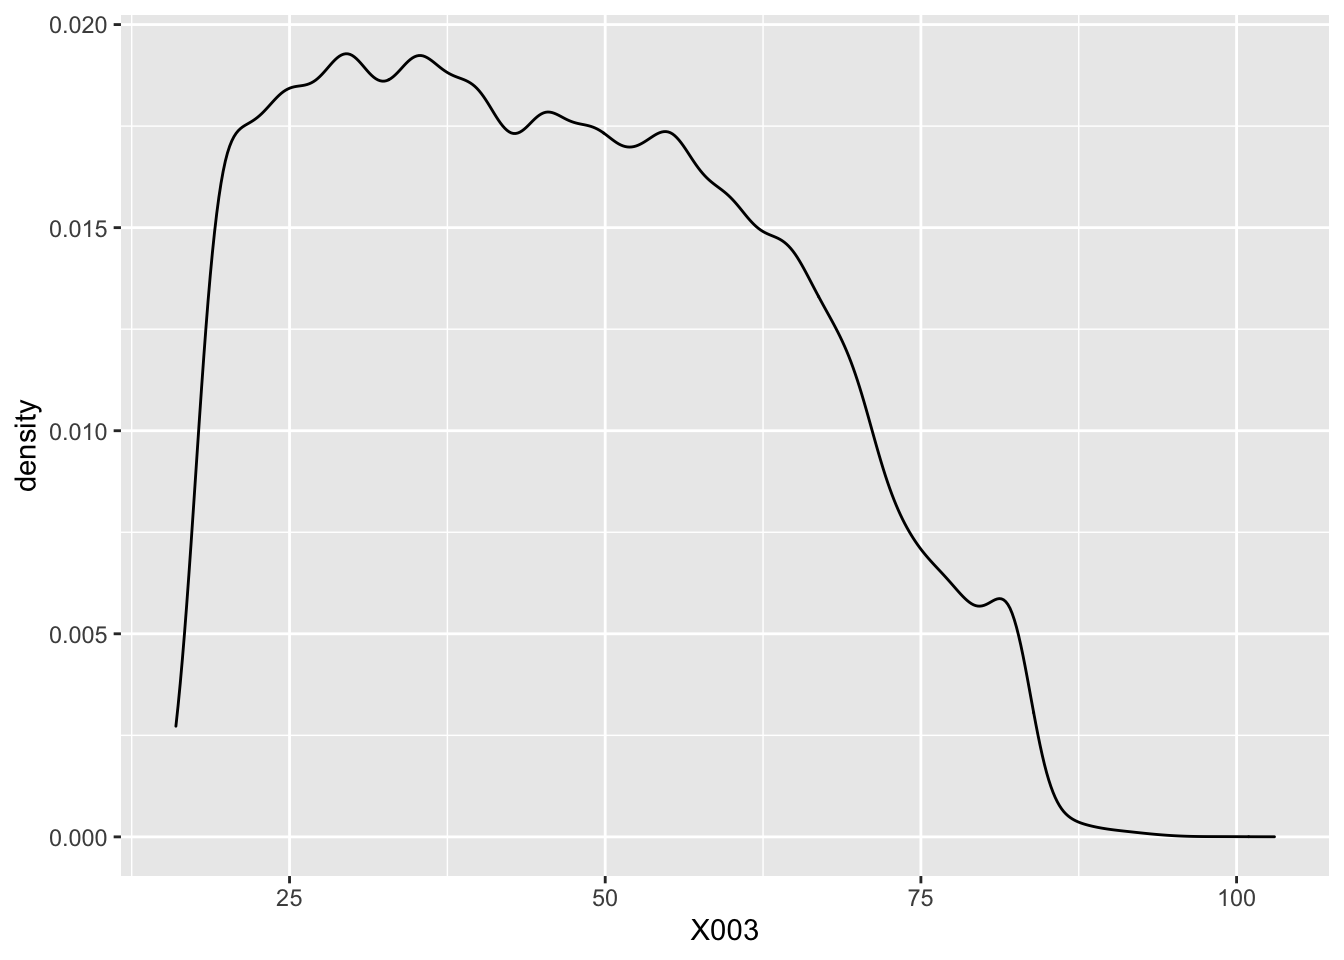
\includegraphics{tutorial_wvsR_files/figure-latex/densidade-1.pdf}

Exemplo 2: aqui, reproduzimos o mapa cultural de Inglehart e Welzel \citeyearpar{inglehart_modernization_2005} para alguns países. Antes, é preciso fazer algumas manipulações com os dados com o que aprendemos nos capítulos anteriores.

\begin{Shaded}
\begin{Highlighting}[]
\CommentTok{# Criar uma lista com os países que se quer analisar}
\CommentTok{# 76=Brasil, 32=Chile, 152=Argentina, 170=Colombia}
\NormalTok{paises <-}\StringTok{ }\KeywordTok{c}\NormalTok{(}\DecValTok{76}\NormalTok{, }\DecValTok{32}\NormalTok{, }\DecValTok{152}\NormalTok{, }\DecValTok{170}\NormalTok{)  }

\CommentTok{# Extrair e retrabalhar as variáveis que precisamos}
\CommentTok{# select() para selecionar as variáveis de interesse}
\CommentTok{# filter() para filtrar usando o vetor 'países' criado acima}
\CommentTok{# group_by() para agrupar por onda-país, onda e país}
\CommentTok{# summarise() para agregar os dados pela média}
\NormalTok{df_y001 <-}\StringTok{ }\NormalTok{df_wvs7 }\OperatorTok
\StringTok{  }\KeywordTok{select}\NormalTok{(S024, S020, S003, tradrat5, survself) }\OperatorTok\StringTok{ }
\StringTok{  }\KeywordTok{filter}\NormalTok{(S003 }\OperatorTok\StringTok{ }\NormalTok{paises) }\OperatorTok\StringTok{ }
\StringTok{  }\KeywordTok{group_by}\NormalTok{(S024, S020, S003) }\OperatorTok\StringTok{ }
\StringTok{  }\KeywordTok{summarise}\NormalTok{(}\DataTypeTok{tradrat5 =} \KeywordTok{mean}\NormalTok{(tradrat5, }\DataTypeTok{na.rm =}\NormalTok{ T),}
            \DataTypeTok{survself =} \KeywordTok{mean}\NormalTok{(survself, }\DataTypeTok{na.rm =}\NormalTok{ T)) }
\end{Highlighting}
\end{Shaded}

Feito isso podemos criar a figura:

Lembre-se que o \texttt{ggplot} usa o símbolo \texttt{+} para adicionar cada um dos elementos da figura.

\begin{Shaded}
\begin{Highlighting}[]
\CommentTok{# lembre se de carregar a variável ggplot se ela não tiver sido carregada }
\KeywordTok{library}\NormalTok{(ggplot2)}

\CommentTok{# Reproduzir o Mapa Cultural Inglehart}

\KeywordTok{ggplot}\NormalTok{(df_y001, }\KeywordTok{aes}\NormalTok{(}\DataTypeTok{x =}\NormalTok{ survself, }
                    \DataTypeTok{y =}\NormalTok{ tradrat5, }
                    \DataTypeTok{color =} \KeywordTok{as.factor}\NormalTok{(S003), }
                    \DataTypeTok{label =} \KeywordTok{as.factor}\NormalTok{(S003))) }\OperatorTok{+}\StringTok{ }
\StringTok{  }\CommentTok{# definir os dados e as dimensões}
\StringTok{  }\KeywordTok{geom_point}\NormalTok{() }\OperatorTok{+}\StringTok{ }\CommentTok{# geometria pontos}
\StringTok{  }\KeywordTok{geom_text}\NormalTok{(}\DataTypeTok{hjust =} \DecValTok{0}\NormalTok{, }\DataTypeTok{nudge_x =} \FloatTok{0.05}\NormalTok{, }\DataTypeTok{check_overlap =} \OtherTok{TRUE}\NormalTok{) }\OperatorTok{+}\StringTok{ }\CommentTok{# rótulos dos pontos}
\StringTok{  }\KeywordTok{scale_x_continuous}\NormalTok{(}\DataTypeTok{limits =} \KeywordTok{c}\NormalTok{(}\OperatorTok{-}\DecValTok{2}\NormalTok{, }\DecValTok{2}\NormalTok{)) }\OperatorTok{+}\StringTok{ }\CommentTok{# restringe eixo x e y entre -2 e 2}
\StringTok{  }\KeywordTok{scale_y_continuous}\NormalTok{(}\DataTypeTok{limits =} \KeywordTok{c}\NormalTok{(}\OperatorTok{-}\DecValTok{2}\NormalTok{, }\DecValTok{2}\NormalTok{)) }\OperatorTok{+}
\StringTok{  }\KeywordTok{labs}\NormalTok{(}\DataTypeTok{x =} \StringTok{"sobrevivencia-autoexpressão"}\NormalTok{,}
       \DataTypeTok{y =} \StringTok{"tradicional-racional"}\NormalTok{,}
       \DataTypeTok{title =} \StringTok{"Mapa Cultural do Inglehart (Brasil, Chile, Argentina, Colombia)"}\NormalTok{) }\CommentTok{# rótulos do gráfico x, y e título}
\end{Highlighting}
\end{Shaded}

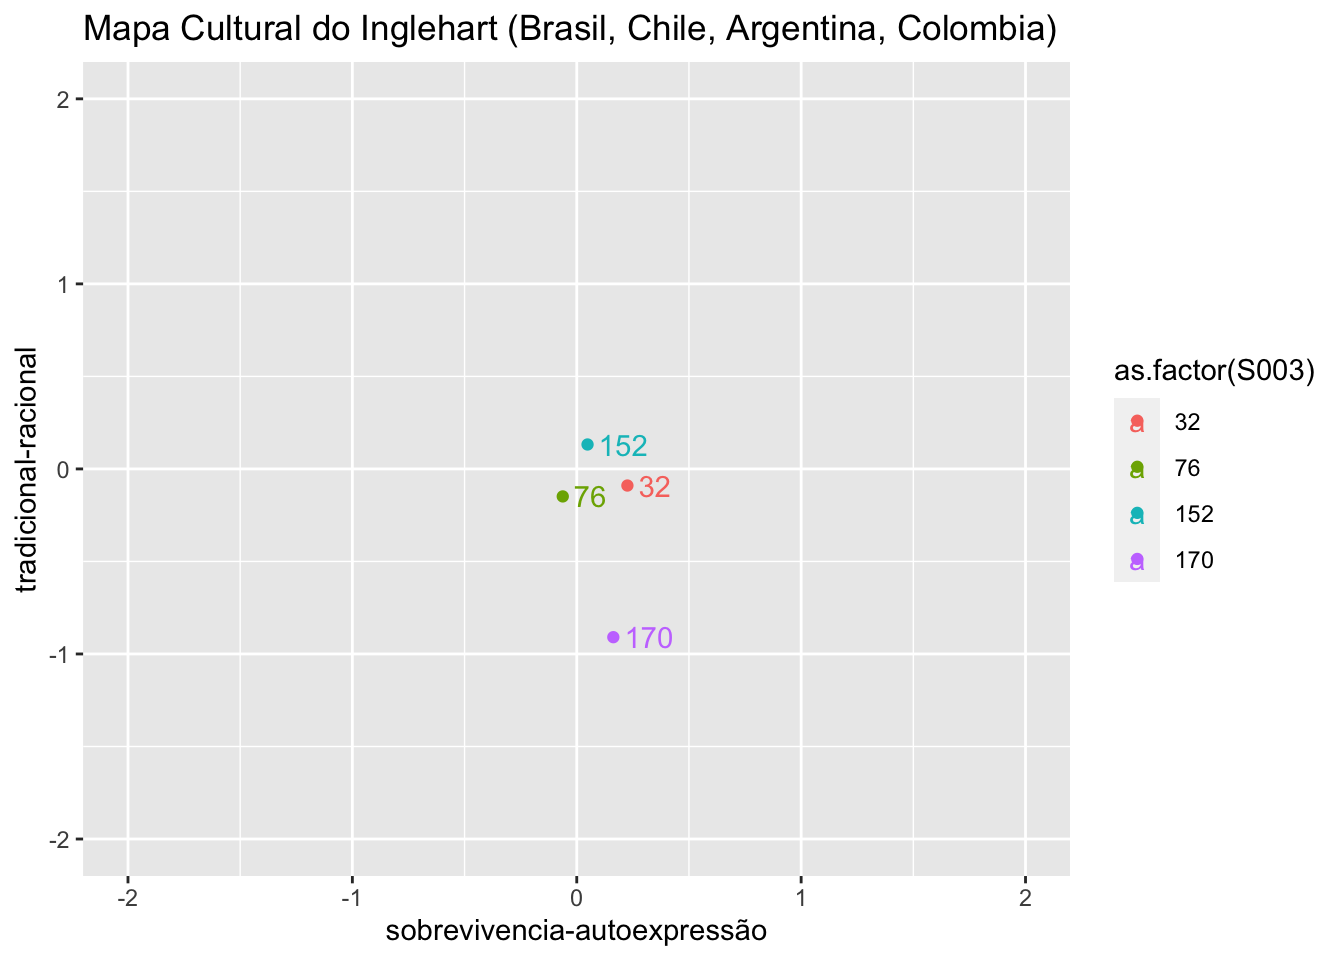
\includegraphics{tutorial_wvsR_files/figure-latex/mapacultural-1.pdf}

\hypertarget{glossuxe1rio}{%
\chapter{Glossário}\label{glossuxe1rio}}

\begin{itemize}
\item
  Programação: alguns conceitos relevantes para aprender uma linguagem de programação.

  \begin{itemize}
  \tightlist
  \item
    Variável: representa um local de armazenamento na memória, com um nome e um valor, mas que não é o valor em si, porque esse pode ser constantemente alterado. Cada variável possui diferentes propriedades, por exemplo, pode ser numérica (\emph{integral} or \emph{double}) ou uma cadeia de caracteres (\emph{string}). Inserindo uma metáfora: cada variável é uma caixinha que pode ter diferentes características (grande, pequena, quadrada, redonda) e que guarda alguma coisa. \texttt{x\ \textless{}-\ 2\ \#cria\ variável\ "x"\ e\ atribuir\ valor\ 2}
  \item
    Objeto: cada objeto é único, específico, e pode ser referenciado. Seu conteúdo pode ser atribuído diretamente ou ser o resultado de uma operação. Cada objeto pode ser armazenado em uma variável. Na metáfora, um objeto pode ser uma carta, uma moeda, um lápis-de-cor. \texttt{y\ \textless{}-\ 5\ \#criar\ objeto\ com\ nome\ y\ e\ atribuir\ valor\ 5}
  \item
    Vetor: uma sequência ordenada de elementos. Importante notar que um vetor armazena apenas um tipo de informação, por exemplo, só números, o que se chama de unidimensional. Como se fosse uma caixinha com várias cartas (uma de fulano, outra de beltrano etc) ou uma caixinha com várias moedas (1 euro, 50 centavos de dólar, 25 centavos de real etc.), uma caixinha com diferentes lápis-de-cor (rosa, azul, verde), ou ainda uma caixinha com moedas e lápis-de-cor. \texttt{z\ \textless{}-\ c(1,\ 2,\ 3)\ \#criar\ vetor\ z\ e\ atribuir\ os\ valores\ 1,\ 2\ e\ 3}
  \item
    Lista: é como um vetor avançado, pois também é uma sequência de elementos, mas pode guardar diferentes tipos de dados (números, letras etc), ou seja, é multidimensional. Assim, pode ser uma caixinha que guarda tudo junto: cartas, moedas e lápis-de-cor. \texttt{lista\ \textless{}-\ list(idade\ =\ 20,\ “oi”,\ 35,\ “tchau”)\ \#criar\ "lista"\ e\ atribuir\ diferentes\ conteúdos}
  \end{itemize}
\item
  Interfaces: o RStudio possui quatro interfaces, que são as ``pequenas telas'' ou ``janelinhas'' que aparecem ao iniciar o programa. Pensando em uma cozinha, o Source seria a receita, o passo-a-passo; o Console seria o fogão, onde tudo está acontecendo, onde se forma o resultado; e o Environment seria uma mesa, onde estão os ingredientes disponíveis. Os pacotes e arquivos ficam no armário, o Viewer, com os utensílios de cozinha e ingredientes disponíveis.
\item
  Funções: diferentes ``verbos'', tanto do R-base quanto na gramática tidyverse. Realizam diferentes tipos de funções.

  \begin{itemize}
  \tightlist
  \item
    Count: conta quantas vezes aparece aquela variável, por exemplo, numa base de dados, e mostra seu valor. \texttt{count(x)\ \#contar\ a\ quantidade\ da\ variável\ x}
  \item
    Filter: filtrar observações (``cadastros'') baseadas em uma condição. \texttt{filter(x\ ==\ 1)\ \#filtra\ todos\ os\ valores\ de\ x\ e\ deixar\ apenas\ os\ cadastros\ em\ que\ x\ tem\ o\ valor\ 1}
  \item
    Select: selecionar variáveis - no plural -, ou seja, escolher mais de uma variável. \texttt{select(x,\ y,\ z)\ \#selecionar\ as\ variáveis\ x,\ y\ e\ z}
  \item
    Group\_by: agrupar variáveis, por exemplo, em uma base de dados grande, ``juntar'' a partir de um determinado quesito. \texttt{group\_by(país)\ \#juntar\ os\ dados\ com\ base\ nos\ diferentes\ valores\ da\ variável\ país}
  \item
    View: visualiza a operação realizada, normalmente, o R cria uma tabela com o(s) conteúdo(s), ficando mais ``simples'' de enxergar os dados. \texttt{view(objeto)}
  \item
    Summarise: resumir, sintetizar, os dados baseados em uma operação, ou seja, criando uma espécie de atalho. \texttt{summarize(media\ =\ mean(idade))\ \#tem\ a\ média\ das\ idades\ das\ pessoas\ como\ critério\ para\ resumir\ ou\ sintetizar\ os\ dados}
  \item
    Mutate: criar nova informação com base em outras. Visualmente, é como se criasse uma nova ``coluna''. \texttt{view(a\ =\ b\ +\ c)\ \#a\ ‘coluna’\ a\ vai\ ter\ o\ valor\ da\ soma\ de\ b\ e\ c}
  \end{itemize}
\item
  Códigos-chave:

  \begin{itemize}
  \tightlist
  \item
    \texttt{\#} para fazer comentários, ou seja, escrever anotações sem que elas sejam executadas como códigos.
  \item
    \texttt{\%\textgreater{}\%} para criar um comando no sentido de ``e então'', ou seja, especificar que seja realizado o próximo passo do código em seguida. Dica: clicar \texttt{Ctrl\ +\ Shift\ +\ M}.
  \item
    \texttt{Ctrl\ +\ enter}, ou clicar no botão \texttt{Run}, para ``rodar'', ou seja, executar o código programado/escrito.
  \end{itemize}
\item
  Estatística:

  \begin{itemize}
  \tightlist
  \item
    Variáveis numéricas: quantitativas, podem ser discretas (contagem, ex.: número de filhos) ou contínuas (mensuração, ex.: peso, altura)
  \item
    Variáveis categóricas: qualitativas, podem ser ordinais (quando há ordem, por exemplo, grau de instrução) ou nominais (classificação, por exemplo, sexo, raça)
  \end{itemize}
\end{itemize}

  \bibliography{tutorial.bib}

\end{document}
